\documentclass[12pt,a4paper]{article}
\usepackage[utf8]{inputenc}
\usepackage[T1]{fontenc}
\usepackage[english]{babel}
\usepackage{fancyhdr}
\usepackage{kpfonts}
\usepackage[margin=1in]{geometry}
\usepackage{exsheets}
\usepackage{amsmath, amssymb, amsfonts}
\usepackage{enumerate}
\usepackage{tikz}
\usetikzlibrary{arrows, decorations.text}

\pagestyle{fancy}
\renewcommand{\headrulewidth}{2pt}
\fancyhead[L]{EPITA\_ING1\_2018\_S6\_PARTIEL\_GREF}
\fancyhead[R]{June 2016}

\fancyfoot[C]{\textbf{\thepage}} 
\fancyfoot[L]{}

\SetupExSheets{solution/print=true}
\SetupExSheets{question/type=exam}
\SetupExSheets[points]{name=point,name-plural=points}
\RenewQuSolPair{question}[name={\large Exercise}]{solution}

\begin{document}
\begin{center}
  
  {\Large \textbf{Networks and Flows on Graphs}}\\

  \vspace{10pt}
  {\Large \textit{Final Exam}}

  \vspace{2\baselineskip}
\end{center}
\begin{center}
\begin{minipage}{\textwidth}
  Duration of the exam : 1h30\\
  No documents are allowed\\
  Only \emph{non-programmable} pocket calculators are allowed\\
  Exercises can be done independently.
\end{minipage}
\end{center}
\rule{\textwidth}{2pt}


\vspace{\baselineskip}
\begin{question}
  The following table sums up $16$ tasks, named from $a$ to $p$, each
  coming with the set of tasks \emph{immediatly} preceding it and the time
  laps it takes to be done.
  \vspace{\baselineskip}
  \begin{displaymath}
    \begin{tabular}{|c|c|c|}
      \hline
      Name of task & Tasks preceding it & Time in weeks \\
      \hline
      a  & -     & 2  \\
      \hline
      b  & a     & 8  \\      
      \hline
      c  & b     & 1  \\      
      \hline
      d  & c     & 3  \\      
      \hline
      e  & d     & 5  \\      
      \hline
      f  & c     & 1  \\      
      \hline
      g  & f     & 2  \\      
      \hline
      h  & c     & 2  \\      
      \hline
      i  & h     & 3  \\      
      \hline
      j  & i     & 8  \\      
      \hline
      k  & e, g  & 7  \\      
      \hline
      l  & k, j  & 2  \\      
      \hline
      m  & l     &  1 \\           
      \hline
      n  & k, j  & 1  \\      
      \hline
     o  & b     &  8 \\      
      \hline
      p  & m, n  & 1  \\             
      \hline
    \end{tabular}
  \end{displaymath}
  \vspace{\baselineskip}
  \begin{enumerate}
  \item Draw the MPM (Meta Potential Model) graph of this project
    planning problem.
  \item Using relevant algorithms, give earliest dates of tasks $a$ to $p$. 
    \begin{itemize}
    \item What is the minimum amount of time the project needs to be done? 
      
    \item What is the critical subgraph of the MPM graph?
    \end{itemize}
  \item Using relevant algorithms, give latest dates of tasks $a$ to $p$.
    \begin{itemize}
    \item What are the margins and free margins of non-critical tasks?
    \end{itemize}
  \end{enumerate}
\end{question}
\begin{question}
  The following graph represents a network through which goes a
  flow. A label $f/c$ corresponds to the flow value $f$ along an
  arrow of capacity $c$.
  \vspace{\baselineskip}
  \begin{center}
    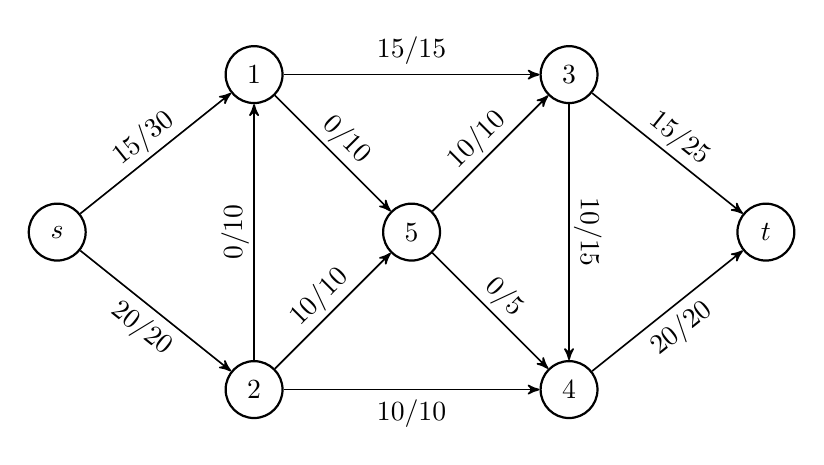
\begin{tikzpicture}
        [minimum width={width("b")+1.5em},
        vertex/.style={circle, draw=black, fill=white, thick},
        arr/.style={->,>=stealth',semithick}]
        \node (t) at (12,5) [vertex] {$t$};
        \node (4) at (9.5,3) [vertex] {$4$}
           edge[
           arr, 
           postaction={
             decorate, 
             decoration={raise=-2.5ex, text along path, text align=center, text={20/20}}
           }
           ] 
           node[below] {} (t);
        \node (3) at (9.5,7) [vertex] {$3$}
           edge[
           arr, 
           postaction={
             decorate, 
             decoration={raise=1ex, text along path, text align=center, text={10/15}}
           }
           ] 
           node[below] {} (4)
           edge[
           arr, 
           postaction={
             decorate, 
             decoration={raise=1ex, text along path, text align=center, text={15/25}}
           }
           ]  node[below] {} (t);
        \node (5) at (7.5,5) [vertex] {$5$}
           edge[
           arr, 
           postaction={
             decorate, 
             decoration={raise=1ex, text along path, text align=center, text={10/10}}
           }
           ] 
           node[above] {} (3)
           edge[
           arr, 
           postaction={
             decorate, 
             decoration={raise=1ex, text along path, text align=center, text={0/5}}
           }
           ]  
           node[above] {} (4);
        \node (1) at (5.5,7) [vertex] {$1$}
           edge[arr] node[above] {$15/15$} (3)
           edge[
           arr, 
           postaction={
             decorate, 
             decoration={raise=1ex, text along path, text align=center, text={0/10}}
           }
           ] 
           node[above] {} (5);
        \node (2) at (5.5,3) [vertex] {$2$}
           edge[arr] node[below] {$10/10$} (4)
           edge[
           arr, 
           postaction={
             decorate, 
             decoration={raise=1ex, text along path, text align=center, text={10/10}}
           }
           ] 
           node[below] {} (5)
           edge[
           arr, 
           postaction={
             decorate, 
             decoration={raise=1ex,text along path, text align=center, text={0/10}}
           }
           ] 
           node[below] {} (1);
        \node (s) at (3,5) [vertex] {$s$}
           edge[           
           arr, 
           postaction={
             decorate, 
             decoration={raise=1ex, text along path, text align=center, text={15/30}}
           }
           ] 
           node[above] {} (1)
           edge[
           arr, 
           postaction={
             decorate, 
             decoration={raise=-2.5ex, text along path, text align=center, text={20/20}}
           }
           ] 
           node[below] {} (2);
     \end{tikzpicture}
  \end{center}
  \vspace{\baselineskip}
  Is the given flow of maximum value? If not, using relevant
  algorithms, show how to get a maximal flow and compute its value.
\end{question}
\end{document}

%%% Local Variables:
%%% mode: latex
%%% TeX-master: t
%%% End:
